\newpage
\section{Variational Principle in Fluid Mechanics}
\subsection{Overview: Cauchy's Equation of Motion}
The equation of motion of a point mass is given by Newton's second law:
\begin{align}
  m \odv[2]{\vec{r}}{t} = \vec{F}
\end{align}
The equation of motion of a fluid (in general) is given by Cauchy's equation of motion:
\begin{align}
  \int_V \rho \odif{V} \, \mdv{\vec{u}}{t} & = \oint_S \odif{S} \, \sigma \vec{n}  + \int_V \rho \odif{V} \, \vec{\tilde{F}}
\end{align}
where
\begin{itemize}
  \item $V$: Volume of the fluid
  \item $S$: Surface of $V$
  \item $\rho (\vec{r}, t)$: Density of the fluid at position $\vec{r}$ and time $t$
  \item $\vec{u} (\vec{r}, t)$: Velocity of the fluid at position $\vec{r}$ and time $t$
  \item $\vec{n}$: Normal vector of the surface $S$ pointing outward
  \item $\sigma (\vec{r}, t)$: Stress tensor of the fluid
  \item $\vec{\tilde{F}}$: External force per unit volume acting on the infinitisimal volume $\odif{V}$ of fluid
\end{itemize}
the stress tensor shows how the forces act on any surface within a fluid.
\begin{align}
  \sigma & = \begin{pmatrix}
               \sigma_{xx} & \sigma_{xy} & \sigma_{xz} \\
               \sigma_{yx} & \sigma_{yy} & \sigma_{yz} \\
               \sigma_{zx} & \sigma_{zy} & \sigma_{zz}
             \end{pmatrix}
\end{align}

The Newtonian derivation of Cauchy's equation of motion is based on the conservation of the momentum of a fluid element:
\begin{align}
  (\pdv{p}{t} + \Delta p \text{ flux per time}) & =
  \begin{multlined}[t]
    (\Delta p \text{ from the surface force}) \\
    + (\Delta p \text{ from the volume force})
  \end{multlined}                                                                       \\
  \implies \quad \rho \odif{V} \mdv{\vec{u}}{t} & = \nabla \cdot (\sigma \vec{n}) + \rho \odif{V} \vec{\tilde{F}}
\end{align}


\cite{eman-fluidEoM}

\subsection{Lagrange Derivative}
Imagine that you want to measure the height of the water in a river at a certain point and time.
Let us assume that you put a very light, small box with some measuring equipment on the water surface at some point $\vec{r}_i$ at time $t_i$.
Then we put another box at another point $\vec{r}_f$ at the same time $t_i$, but we fix this box so that it does not move.

\begin{wrapfigure}{r}{0.5\textwidth}
  \centering
  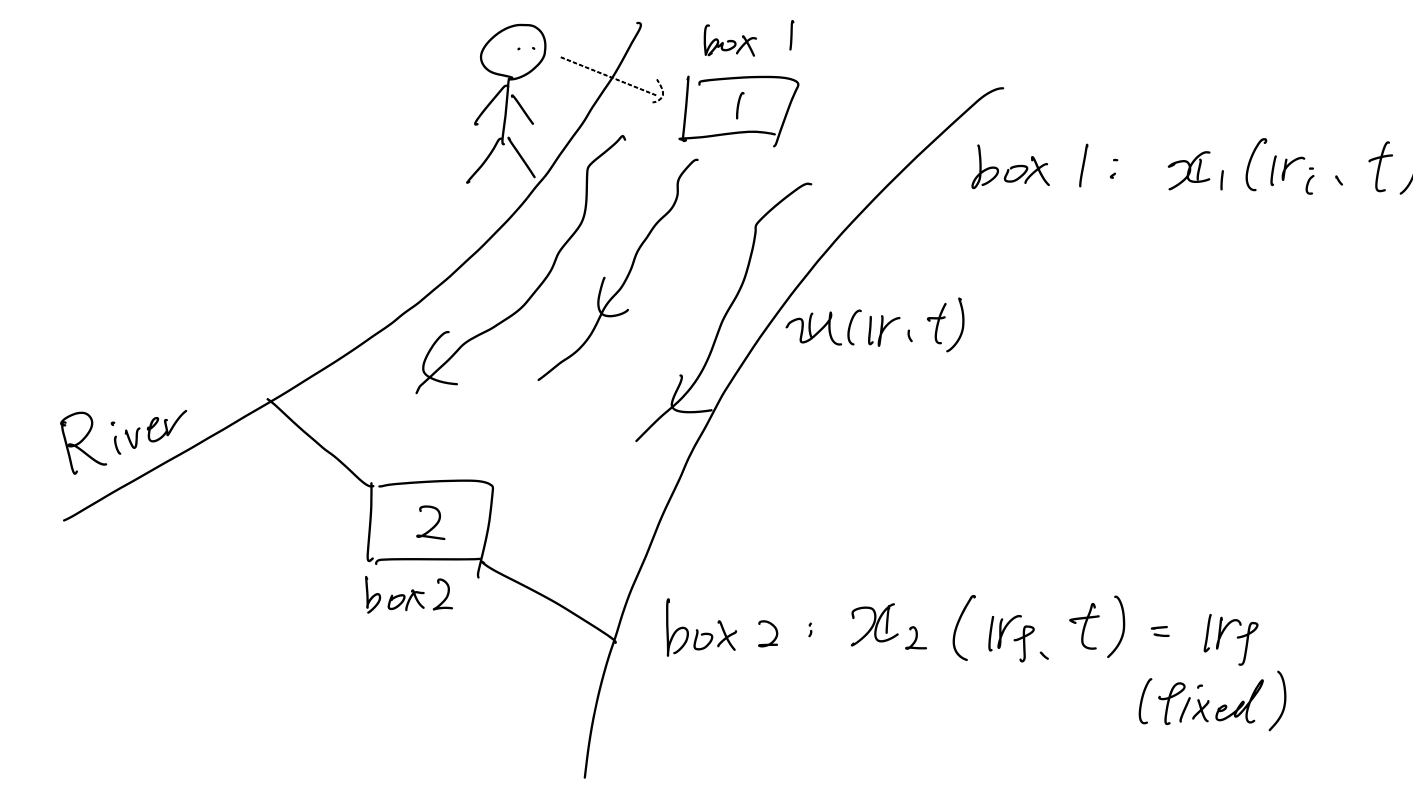
\includegraphics[width=0.45\textwidth]{images/am/river.png}
  \caption{Boxes on a river}
  \label{fig:lagrange_derivative}
\end{wrapfigure}
Since the water surface is not static, box 1 will be carried by the water flow.
Let us denote the position of the box 1 at time $t$ as $\vec{\xi} (\vec{r}_i, t; t_i)$, where the box 1 is placed at the point $\vec{r}_i$ at time $t_i$.

Let us denote the height of the water surface at a point $\vec{r}$ at time $t$ by $X(\vec{r}, t)$.
Then, we can write the height of the water surface at the positions of box 1 and 2 at time $t$ as
\begin{align}
  X(\vec{\xi}, t) & = X_1(t) \\
  X(\vec{r}_f, t) & = X_2(t)
\end{align}
Finally, assume that the box 1 will reach $\vec{r}_f$ at time $t_f$.

Now, at initial time $t_i$, the change in height of the water surface is given by:
\begin{align}
  X(\vec{r}_f, t_i) - X(\vec{r}_i, t_i) & = \nabla X(\vec{r}_i, t_i) \cdot (\vec{r}_f - \vec{r}_i) \\
                                        & = \nabla X(\vec{r}_i, t_i) \cdot \Delta \vec{r}
\end{align}
assuming that $\Delta \vec{r} := \vec{r}_f - \vec{r}_i$ is small enough.
On the other hand, for box 2, the change in height of the water surface in a time interval $\Delta t = t_f - t_i$ is given by:
\begin{align}
  X(\vec{r}_f, t_f) - X(\vec{r}_f, t_i) & = \pdv{X(\vec{r}_f, t_i)}{t} \Delta t
\end{align}
Thus, the total change of $X$ measured by box 1, during $\Delta t$, moving at the velocity $\vec{u}$ is given by
\begin{align}
  X(\vec{r}_f, t_f) - X(\vec{r}_i, t_i)
   & = X(\vec{r}_f, t_f) \underbrace{
    - X(\vec{r}_f, t_i)
    + X(\vec{r}_f, t_i)
  }_{=0} - X(\vec{r}_i, t_i)                                               \\
   & = \pdv{X}{t} \Delta t + \nabla X(\vec{r}_i, t_i) \cdot \Delta \vec{r}
\end{align}
Now, since $\vec{r}_i = \vec{\xi}(\vec{r}_i, t_i)$ and $\vec{r}_f = \vec{\xi}(\vec{r}_i, t_f)$, we can rewrite the equation above:
\begin{align}
  X(\vec{\xi}(\vec{r}_i, t_f), t_f) - X(\vec{\xi}, t_i) & = \pdv{X}{t} \Delta t + \nabla X(\vec{\xi}, t_i) \cdot \Delta \vec{\xi}
\end{align}
where $\Delta \vec{\xi} = \vec{\xi}(\vec{r}_i, t_f) - \vec{\xi}(\vec{r}_i, t_i)$.

Using $\Delta t = t_f - t_i$, we can rewrite the equation above as:
\begin{align}
  \frac{X(\vec{\xi} + \Delta \vec{\xi}, t_i + \Delta t) - X(\vec{\xi}, t_i)}{\Delta t}
   & = \pdv{X}{t} + \nabla X(\vec{\xi}, t_i) \cdot \frac{\Delta \vec{\xi}}{\Delta t} \\
\end{align}
Since the box 1 is a part of the fluid, the time derivative of $\vec{\xi}$ is the velocity of the fluid at the position $\vec{\xi}$:
\begin{align}
  \pdv{\vec{\xi}(\vec{r}_i, t)}{t} & = \vec{u}(\vec{\xi}, t)
\end{align}
\nt{
  In this derivative, we fix the starting position $\vec{r}_i$, we only care about the time evolution from the position $\vec{r}_i$.
  This is different from the total derivative, which takes into account a change in the starting position $\vec{r}_i$.
}
thus, by taking $\Delta t \to 0 (\implies \Delta x \to 0)$, we can rewrite the equation above as:
\begin{align}
  \mdv{X(\vec{\xi}, t_i)}{t} & := \pdv{X(\vec{\xi}, t_i)}{t} + \vec{u}(\vec{\xi}, t_i) \cdot  \nabla X(\vec{\xi}, t_i)
\end{align}
where $\mdv{}{t}$ indicates that we are tracking the box 1 and its measurement of $X$.
This is called the \emph{Lagrange derivative}:
\dfn{Lagrange Derivative}{
  The Lagrange description in Eulerian perspective is given as the \emph{Lagrange derivative}:
  \begin{align}
    \mdv{X}{t} := \pdv{X}{t} + \vec{u} \cdot \nabla X
  \end{align}
  which tracks the change of a physical quantity $X$ with the flow.
}

Now, define a new quantity called the "position function" $\vec{x}(\vec{r}, t)$:
\begin{align}
  \vec{x}(\vec{r}, t) & := \vec{r}
\end{align}
If we measure this position function at the box 1 at $t = t_i$,
\begin{align}
  \vec{x}(\vec{r}_i, t_i) & = \vec{r}_i
\end{align}
and notice that tracking the position of box 1 is equivalent to observing the time-evolved position $\xi(\vec{r}_i, t_i)$:
\begin{align}
  \pdv{\vec{\xi}}{t} & = \mdv{\vec{x}}{t} = \vec{u}(\vec{x}, t)
\end{align}

\subsection{Derivation from Action Integral}
In Newtonian mechanics, for a particle of mass $m$, the action integral $S$ is given by:
\begin{align}
  S & = \int \odif{t} \, L = \int \odif{t} \, m \lagr, \quad \lagr := \frac{L}{m} = \bab{\frac{1}{2} \dot{\vec{x}}^{\, 2} - \tilde{V}(\vec{x})}
\end{align}
where $\lagr$ is the Lagrangian density, and
\begin{align}
  \tilde{V}(\vec{x}) & = \frac{V(\vec{x})}{m}
\end{align}
by assuming a similar form of the Lagrangian density for a fluid, we can write the action integral for a fluid as:
\begin{align}
  S & = \int \odif{t} \, L = \int \odif{t} \, \int_V \rho(\vec{x}, t) \odif{V}(\vec{x}, t) \, \lagr\pab{\vec{x}, \mdv{\vec{x}}{t}}
\end{align}
where the Lagrangian density is
\begin{align}
  \lagr \pab{\vec{x}(\vec{r}, t), \mdv{\vec{x}(\vec{r}, t)}{t}} & = \frac{1}{2} \pab{\mdv{\vec{x}(\vec{r}, t)}{t}}^2 - \tilde{V}(\vec{x}(\vec{r}, t)) + \frac{1}{\rho(\vec{r}, t)} \nabla \cdot \sigma(\vec{r}, t) \vec{x}(\vec{r}, t)
\end{align}
Then the Euler-Lagrange equation for this Lagrangian density is given by:
\begin{align}
  \pdv{\lagr}{\vec{x}} - \mdv{}{t} \pab{\pdv{\lagr}{\pab{\mdv{\vec{x}}{t}}}} & = 0
\end{align}
calculating the partial derivative gives:
\begin{align}
  \pdv{\lagr}{\vec{x}}                & = \frac{1}{\rho} \nabla \cdot \sigma - \nabla \tilde{V}(\vec{x}) = \frac{1}{\rho} \nabla \cdot \sigma + \vec{\tilde{F}} \\
  \pdv{\lagr}{\pab{\mdv{\vec{x}}{t}}} & = \mdv{\vec{x}}{t} = \vec{u}(\vec{x}, t)
\end{align}
hence the Euler-Lagrange equation becomes:
\begin{align}
  \mdv{\vec{u}}{t} & = \frac{1}{\rho} \nabla \cdot \sigma + \vec{\tilde{F}}
\end{align}
by integrating over the volume $V$, we get
\begin{align}
  \int_V \rho \odif{V} \, \mdv{\vec{u}}{t}                & = \int_V \odif{V} \, \nabla \cdot \sigma + \int_V \rho \odif{V} \, \vec{\tilde{F}}  \\
  \implies \quad \int_V \rho \odif{V} \, \mdv{\vec{u}}{t} & = \int_V \odif{s} \, \vec{n} \cdot \sigma + \int_V \rho \odif{V} \, \vec{\tilde{F}}
\end{align}


\subsection{Hamilton Formalism}
Similarly to the point mass case, we should define the momentum density $\vec{\pi}(\vec{r}, t)$ as the derivative of the Lagrangian density with respect to the velocity:
\begin{align}
  \vec{\pi} (\vec{r}, t) & = \pdv{\lagr}{\pab{\mdv{\vec{x}}{t}}}
\end{align}
then the Hamiltonian density should be defined by the Legendre transformation:
\begin{align}
  \hami(\vec{\pi}, \vec{x}) & = \vec{\pi} \cdot \mdv{\vec{x}}{t} - \lagr \pab{\vec{x}, \mdv{\vec{x}}{t}}                               \\
                            & = \frac{1}{2} \pab{\mdv{\vec{x}}{t}}^2 + \tilde{V}(\vec{x}) - \frac{1}{\rho} \nabla \cdot \sigma \vec{x}
\end{align}


\cite{suzuki-leastActionFluid}



